\documentclass[tikz,border=2pt]{standalone}
\renewcommand{\familydefault}{\sfdefault}
\usetikzlibrary{arrows.meta,calc,positioning}
\tikzset{every picture/.style={line width=1pt, >=Stealth},
         hl/.style={fill=black, fill opacity=0.12, text opacity=1}}
\begin{document}
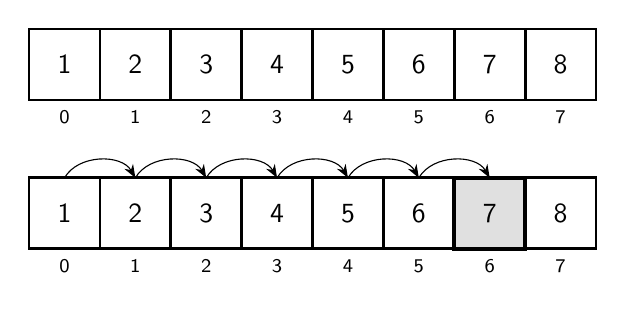
\begin{tikzpicture}[x=0.9cm, y=0.9cm, cell/.style={draw, minimum size=0.9cm},
    found/.style={hl, line width=1.6pt}]
  % \row{y}{value/style, ...}: one array, with each index below its cell
  \newcommand{\row}[2]{\foreach \v/\s [count=\i from 0] in {#2} {
    \node[cell, \s] at (\i, #1) {\v};
    \node[font=\scriptsize] at (\i, #1 - 0.75) {\i};
  }}
  \row{0}{1/,2/,3/,4/,5/,6/,7/,8/}
  \foreach \i in {0,...,5} \draw[->, thin] (\i, -1.6) to[bend left=60] (\i+1, -1.6);
  \row{-2.1}{1/,2/,3/,4/,5/,6/,7/found,8/}
\end{tikzpicture}
\end{document}
